% !TEX root = poster.tex
\headerbox{\textbf{Calibration}}{name=calib,column=0,row=1,below=basics,above=bottom}{
\textbf{Mistag calibration}
\vspace{-0.6em}
\begin{center}
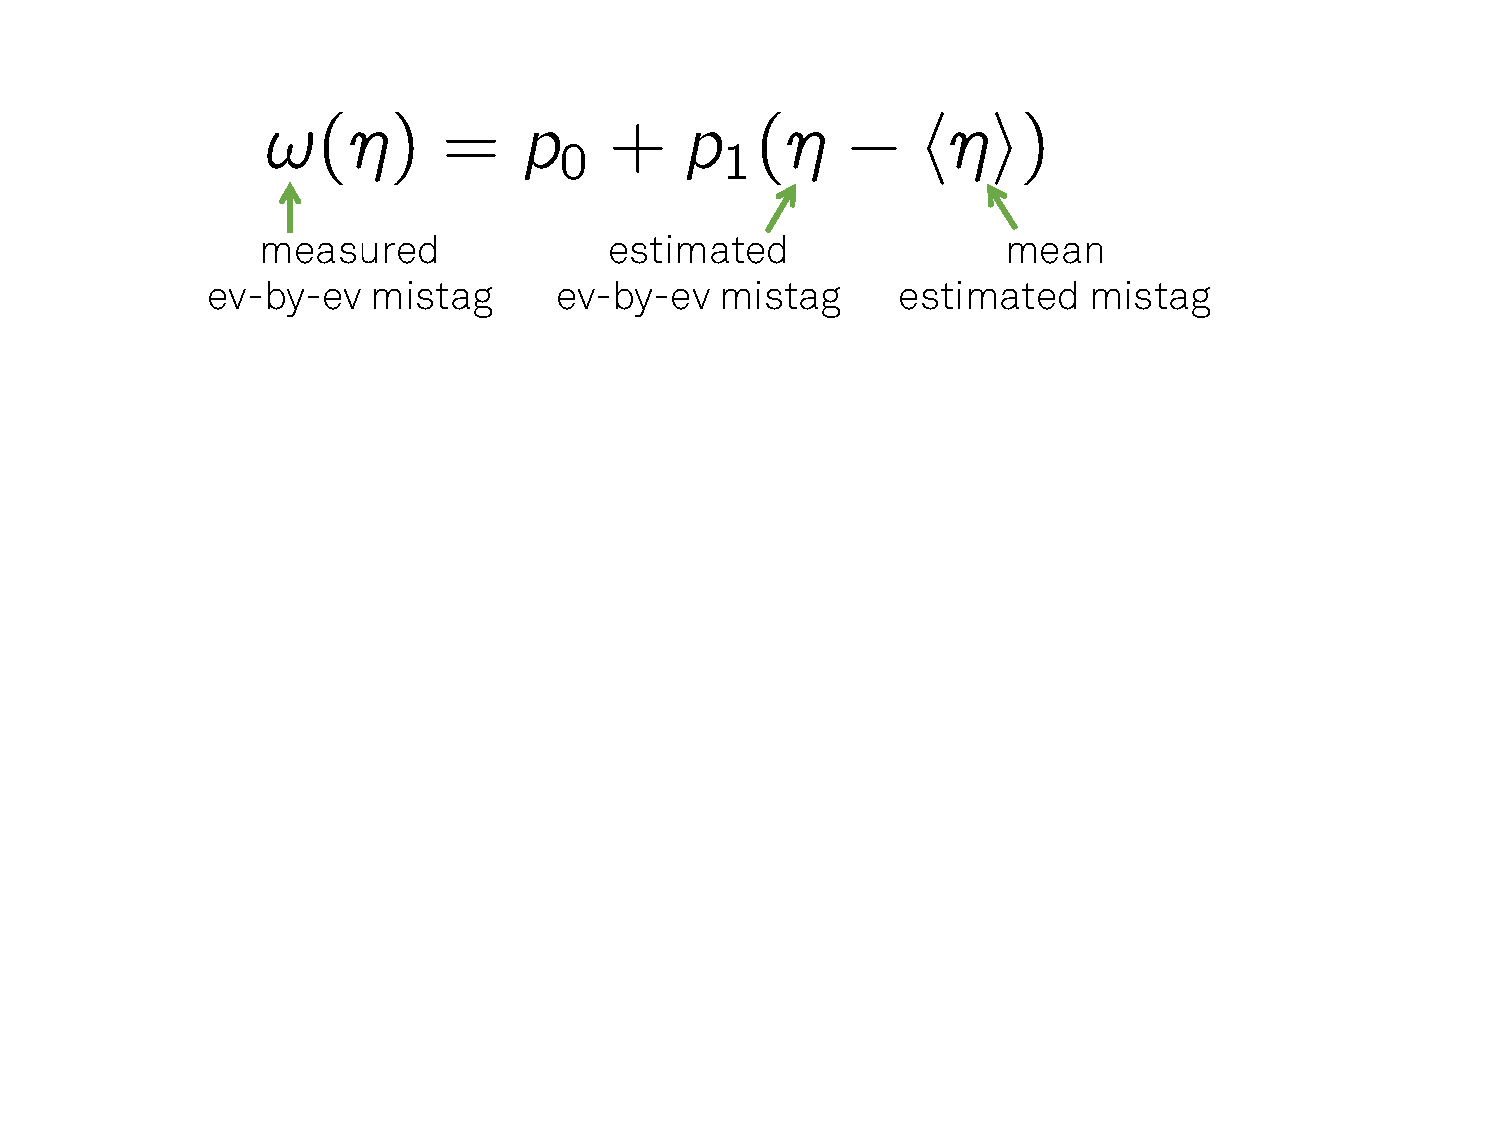
\includegraphics[width=0.75\textwidth]{figures/Calibration.pdf}
\end{center}
\vspace{-0.65em}
Several flavour-specific decay channels are used
\vspace{-0.5em}
\begin{itemize}
\setlength\itemsep{0.01em}
\item \BuToJPsiKp, $\Bu \rightarrow \D^0 \pi^+$ \\[0.05cm]
charged channels: extract $\omega$ by comparing tag decision with charge of the final state
\item \BdToJPsiKst, \BdToDstarmunu, $\Bs \rightarrow D_s^- \pi^+$, ...\\[0.05cm]
neutral channels: full time-dependent analysis to extract $\omega$ from the mixing asymmetry 
%\vspace{-0.1em}
\begin{equation*}
\mathcal{A}_{\text{mix}}(t) \propto (1-2\omega)\cos (\Delta m_{d/s} t)
\end{equation*}
\end{itemize}
\vspace{-1.9em}
\begin{center}
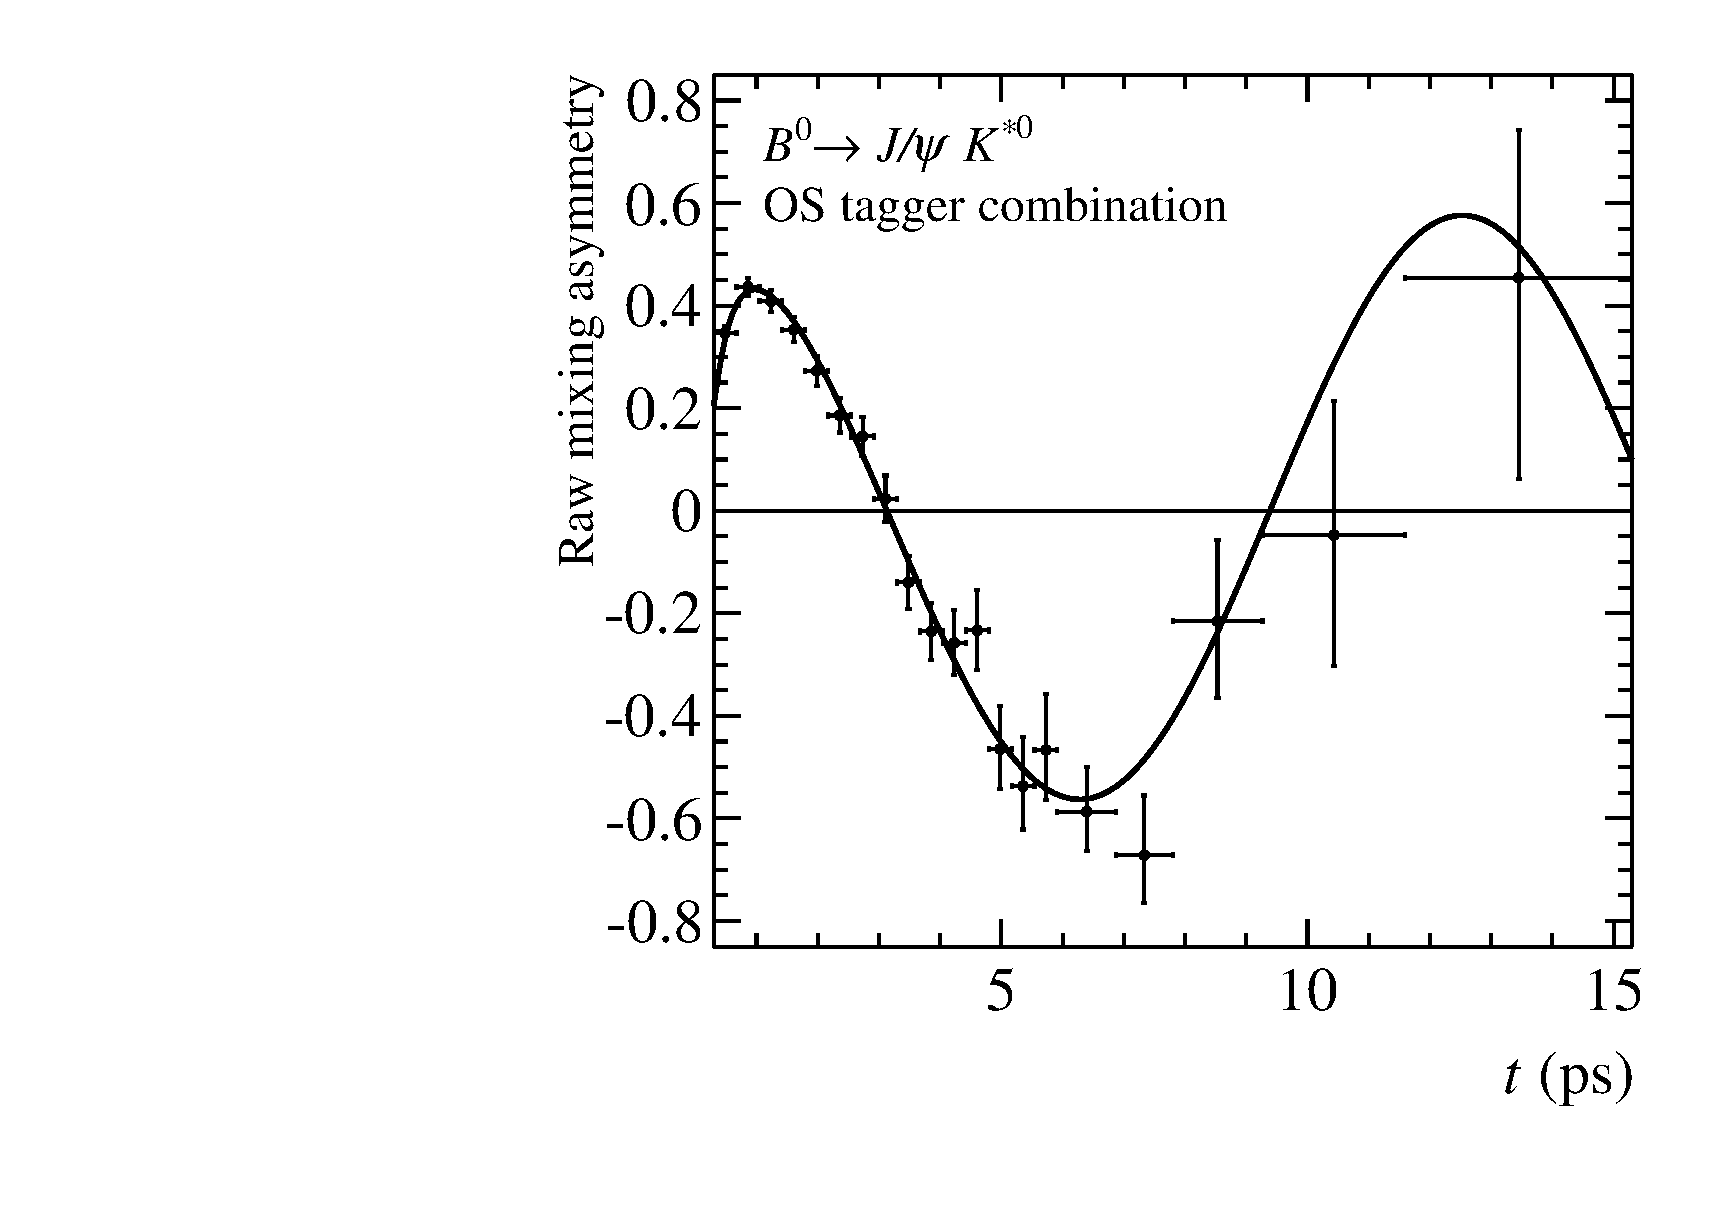
\includegraphics[width=0.475\boxwidth]{KstAsym.pdf}
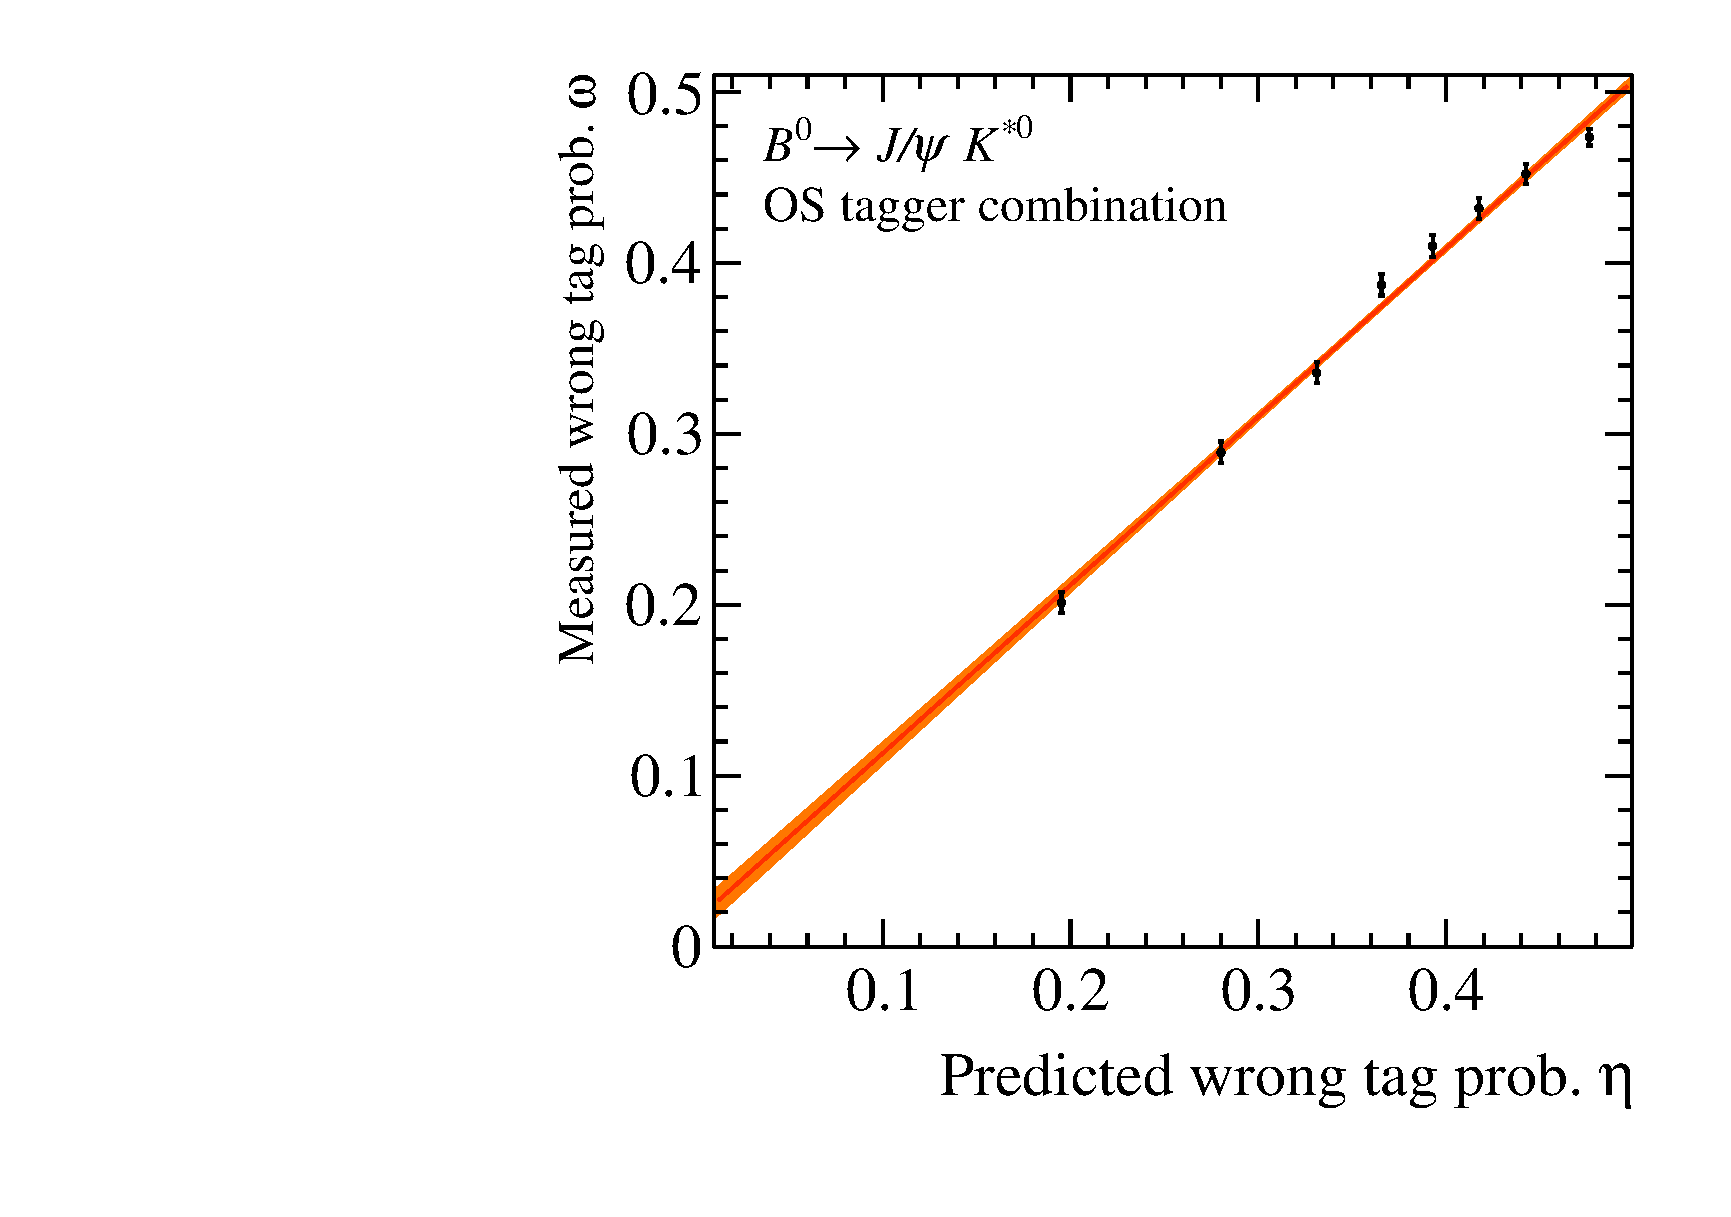
\includegraphics[width=0.475\boxwidth]{Bd2JpsiKst-Kst-OST-8ScalingFunction_raw.pdf}
\end{center}

}